\PassOptionsToPackage{table}{xcolor}
\documentclass[
    aspectratio=169
]{beamer}

\mode<presentation> {
\usetheme{Madrid}
\definecolor{Royalblue}{cmyk}{1, 0.72, 0, 0.38}
\usecolortheme[named=Royalblue]{structure}
\usefonttheme[onlymath]{serif}
}

\usepackage{graphicx}
\usepackage{booktabs}
\usepackage{caption}
\usepackage{multicol}

\setbeamertemplate{navigation symbols}{}
\setbeamertemplate{footline}
{
  \hbox{\begin{beamercolorbox}[wd=1\paperwidth,ht=2.25ex,dp=1ex,right]{framenumber}%
      \usebeamerfont{framenumber}{\color{black}{\insertframenumber{} / \inserttotalframenumber}}\hspace*{2ex}
    \end{beamercolorbox}}%
  \vskip0pt%
}

%----------------------------------------------------------------------------------------
%	TITLE PAGE
%----------------------------------------------------------------------------------------

\title[DICHASUS Fidelity]{{\textbf{Real-World Fidelity Validation}}}

\subtitle{DICHASUS Indoor Channel Measurements vs.\ Ray Tracing}

\author{{\bf{{\large{Namhyun Kim}}}}}
\institute[ASU]
{
{\normalsize{Arizona State University}} \\
{\normalsize{School of Electrical, Computer and Energy Engineering (ECEE)}} \\
\medskip
}
\date{April 2026}

\begin{document}

\begin{frame}
\titlepage
\end{frame}

%------------------------------------------------
\begin{frame}{\textbf{Outline}}
\tableofcontents
\end{frame}

%------------------------------------------------
\section{Motivation}
%------------------------------------------------

\begin{frame}{\textbf{Why Real-World Validation?}}
\begin{block}{Gap in Sim-Only Analysis}
\centering
\large Canyon experiments used \textbf{sim-vs-sim} comparison. \\
Does the fidelity framework hold against \textbf{real measurements}?
\end{block}

\vspace{0.3cm}
\begin{columns}[T]
\begin{column}{0.55\textwidth}
\textbf{Approach}:
\begin{enumerate}
    \item Use DICHASUS \textbf{real indoor measurements} as ground truth.
    \item Apply the same \textbf{4-axis degradation} framework.
    \item Compare RT simulation vs.\ measured CSI at each level.
    \item Validate which thresholds from Canyon still hold.
\end{enumerate}
\end{column}
\begin{column}{0.42\textwidth}
\begin{block}{Key Difference from Canyon}
\begin{itemize}
    \item Ground truth = \textbf{real hardware}, not sim baseline.
    \item Includes real-world effects: noise, calibration, unmodeled scattering.
    \item Much harder benchmark.
\end{itemize}
\end{block}
\end{column}
\end{columns}
\end{frame}

%------------------------------------------------
\section{Dataset and Setup}
%------------------------------------------------

\begin{frame}{\textbf{DICHASUS dc41 Dataset}}
\footnotesize
\begin{columns}[T]
\begin{column}{0.48\textwidth}
\begin{block}{Measurement Setup}
\begin{itemize}
    \item \textbf{Frequency}: 3.438\,GHz, 50\,MHz bandwidth.
    \item \textbf{Antennas}: 64 distributed (2 arrays of 4$\times$8).
    \item \textbf{Subcarriers}: 1024 OFDM.
    \item \textbf{Positions}: 3282 with tachymeter ground truth.
    \item \textbf{Environment}: INUE hallway, University of Stuttgart.
    \item \textbf{Scenario}: No intentional blockers (dc41).
\end{itemize}
\end{block}
\end{column}
\begin{column}{0.48\textwidth}
\begin{block}{3D Scene Variants and RT Setup}
\begin{itemize}
    \item \texttt{inue\_simple}: 3 objects (walls, floor, ceiling).
    \item \texttt{inue\_detailed}: 14 objects (+pillars, doors, glass, mirror).
    \item \texttt{inue\_full}: 22 objects (+blockers, arrays).
    \item Sionna 2.0 PathSolver, baseline depth=5, 500K samples.
    \item 30 positions per config (uniform subsample).
\end{itemize}
\end{block}
\end{column}
\end{columns}
\normalsize
\end{frame}

%------------------------------------------------

\begin{frame}{\textbf{24 Degradation Configs}}
\vspace{-0.1cm}
\begin{columns}[T]
\begin{column}{0.48\textwidth}
\begin{block}{1. Geometry (3 configs)}
\begin{itemize}
    \item Simple scene (3 objects)
    \item Detailed scene, no blockers (14 objects)
    \item Full scene (22 objects)
\end{itemize}
\end{block}
\begin{block}{2. Material (6 configs)}
\begin{itemize}
    \item Baseline (per-object ITU materials)
    \item Uniform override: concrete, metal, glass, plasterboard, wood
\end{itemize}
\end{block}
\end{column}
\begin{column}{0.48\textwidth}
\begin{block}{3. Ray Tracing (9 configs)}
\begin{itemize}
    \item Reflection depth: 1, 2, 3, 5, 7
    \item Ray samples: 5K, 50K, 500K
    \item Diffuse reflection: on
\end{itemize}
\end{block}
\begin{block}{4. Hardware (6 configs)}
\begin{itemize}
    \item Baseline (TR38.901 TX, dipole RX)
    \item TX pattern: dipole, isotropic
    \item Spacing: $0.4\lambda$
    \item Polarization: H
    \item RX pattern: isotropic
\end{itemize}
\end{block}
\end{column}
\end{columns}
\end{frame}

%------------------------------------------------

\begin{frame}{\textbf{Metrics}}
\footnotesize
\begin{columns}[T]
\begin{column}{0.48\textwidth}
\begin{block}{Scaled NMSE}
$$\text{NMSE} = \min_\alpha \frac{\|\alpha \mathbf{h}_\text{sim} - \mathbf{h}_\text{meas}\|^2}{\|\mathbf{h}_\text{meas}\|^2}$$
\vspace{-0.2cm}
\begin{itemize}
    \item Removes global power/phase offset.
    \item $\alpha^* = \langle \mathbf{h}_\text{sim}, \mathbf{h}_\text{meas}\rangle / \langle \mathbf{h}_\text{sim}, \mathbf{h}_\text{sim}\rangle$.
    \item 0\,dB = uncorrelated; $<$0\,dB = useful.
\end{itemize}
\end{block}
\end{column}
\begin{column}{0.48\textwidth}
\begin{block}{Additional Metrics}
\begin{itemize}
    \item \textbf{Spatial power corr.}: antenna power profile similarity.
    \item \textbf{PDP corr.}: power delay profile shape match.
    \item \textbf{RMS delay error}: delay spread difference (ns).
    \item \textbf{Per-antenna CFR corr.}: avg.\ per-antenna frequency response correlation.
\end{itemize}
\end{block}
\end{column}
\end{columns}
\vspace{0.1cm}
\begin{block}{Note}
Unlike Canyon sim-vs-sim (NMSE $\approx -40$\,dB baseline), real-world comparison has an inherent gap from unmodeled effects. We focus on \textbf{relative differences}.
\end{block}
\normalsize
\end{frame}

%------------------------------------------------
\section{Results}
%------------------------------------------------

\begin{frame}{\textbf{Overview: All 24 Configs}}
\begin{center}
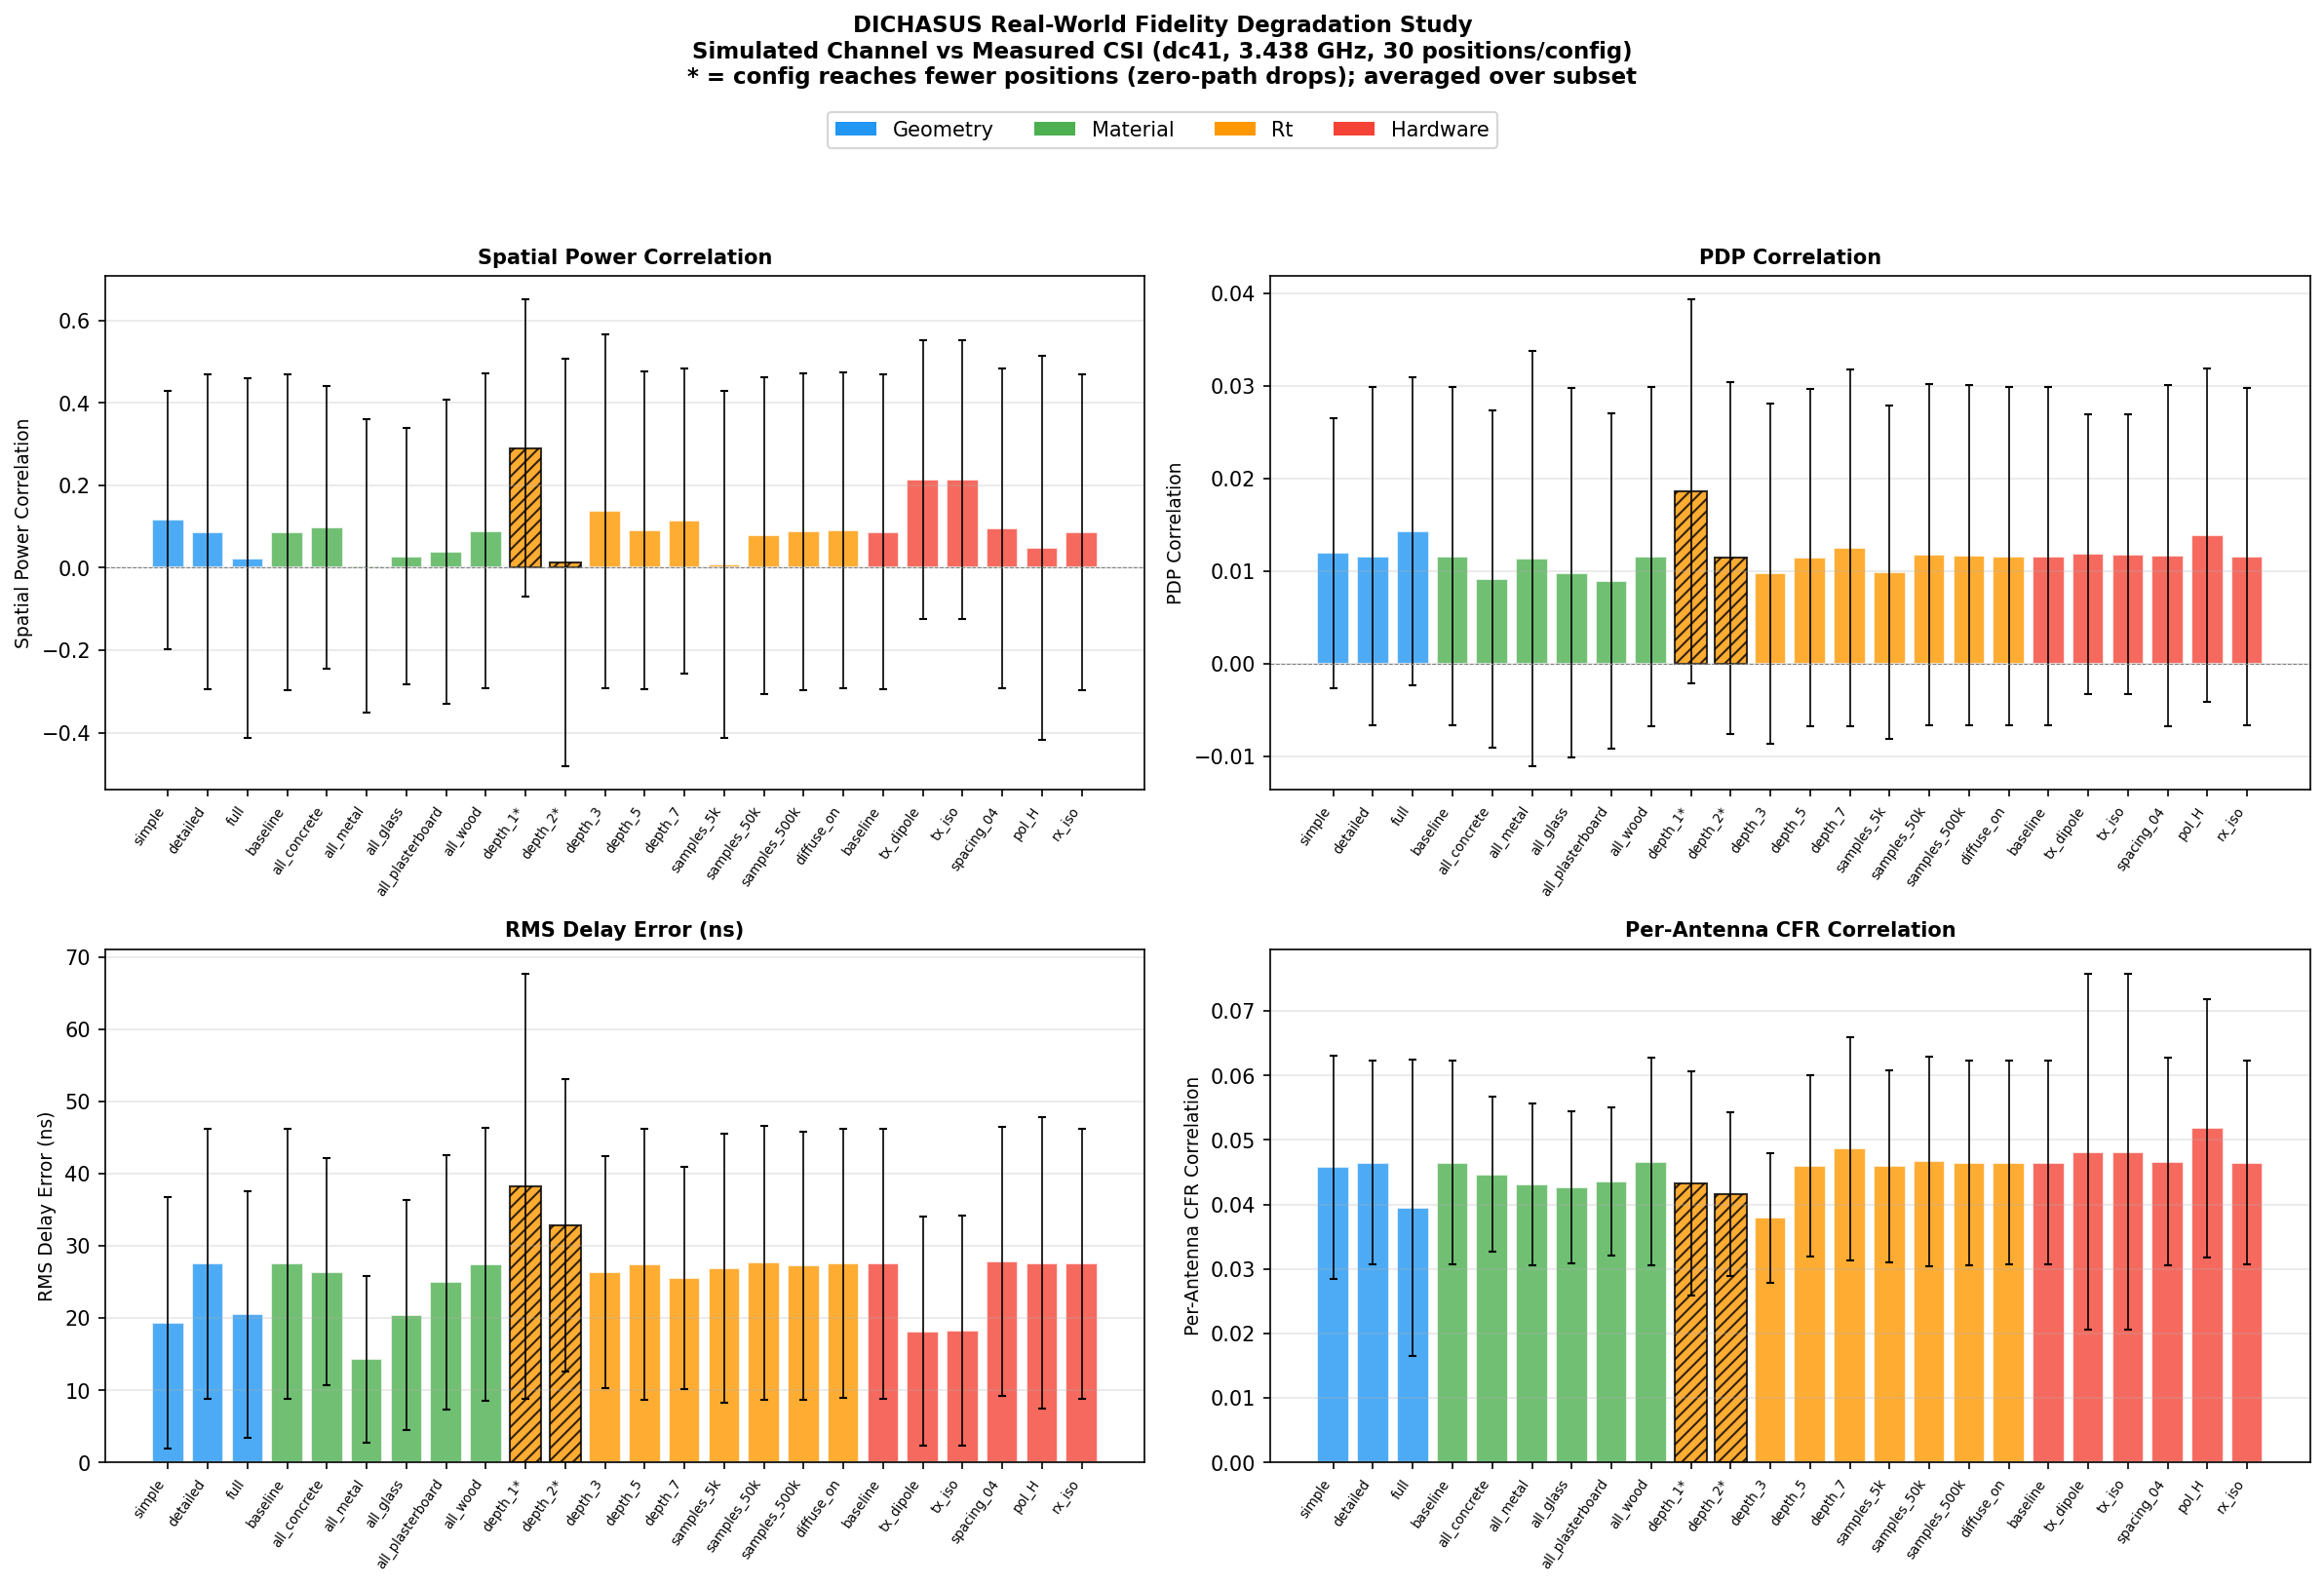
\includegraphics[width=0.95\linewidth,height=0.75\textheight,keepaspectratio]{dichasus_fidelity/fidelity_degradation.png}
\end{center}
\end{frame}

%------------------------------------------------

\begin{frame}{\textbf{Geometry: More Detail $\neq$ Better Match}}
\vspace{-0.2cm}
\begin{columns}[T]
\begin{column}{0.52\textwidth}
\begin{center}
    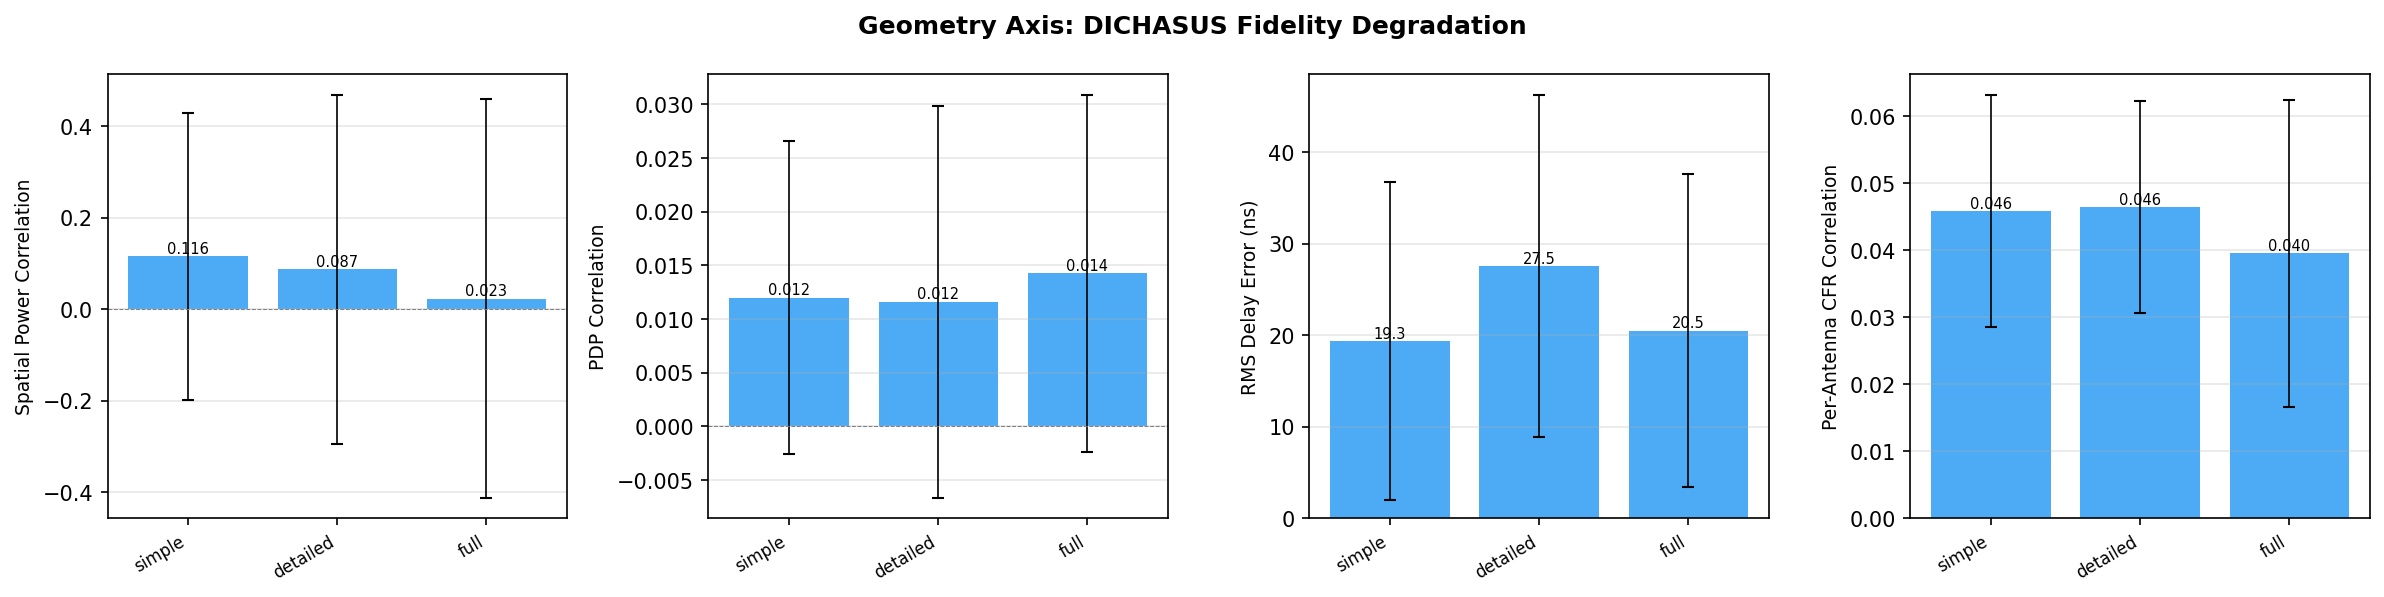
\includegraphics[width=\linewidth,height=0.55\textheight,keepaspectratio]{dichasus_fidelity/geometry_detail.png}
\end{center}
\end{column}
\begin{column}{0.45\textwidth}
\vspace{0.3cm}
\footnotesize
\begin{tabular}{rcc}
\toprule
\textbf{Scene} & \textbf{Pwr Corr} & \textbf{PDP Corr} \\
\midrule
\rowcolor{green!15} Simple & $0.116$ & $0.0120$ \\
Detailed & $0.087$ & $0.0116$ \\
Full & $0.023$ & $0.0143$ \\
\bottomrule
\end{tabular}
\normalsize
\vspace{0.3cm}
\begin{block}{\footnotesize Key Finding}
\footnotesize
Adding geometry detail actually \textbf{hurts} match (0.12 $\to$ 0.09 $\to$ 0.02). More objects create more reflection paths, but without calibrated materials these paths add noise, not signal. PDP correlation is flat ($\sim$0.012) --- scene complexity doesn't touch the fine multipath structure.
\end{block}
\end{column}
\end{columns}
\end{frame}

%------------------------------------------------

\begin{frame}{\textbf{Material: Uniform Override Has Limited Impact}}
\vspace{-0.2cm}
\begin{columns}[T]
\begin{column}{0.52\textwidth}
\begin{center}
    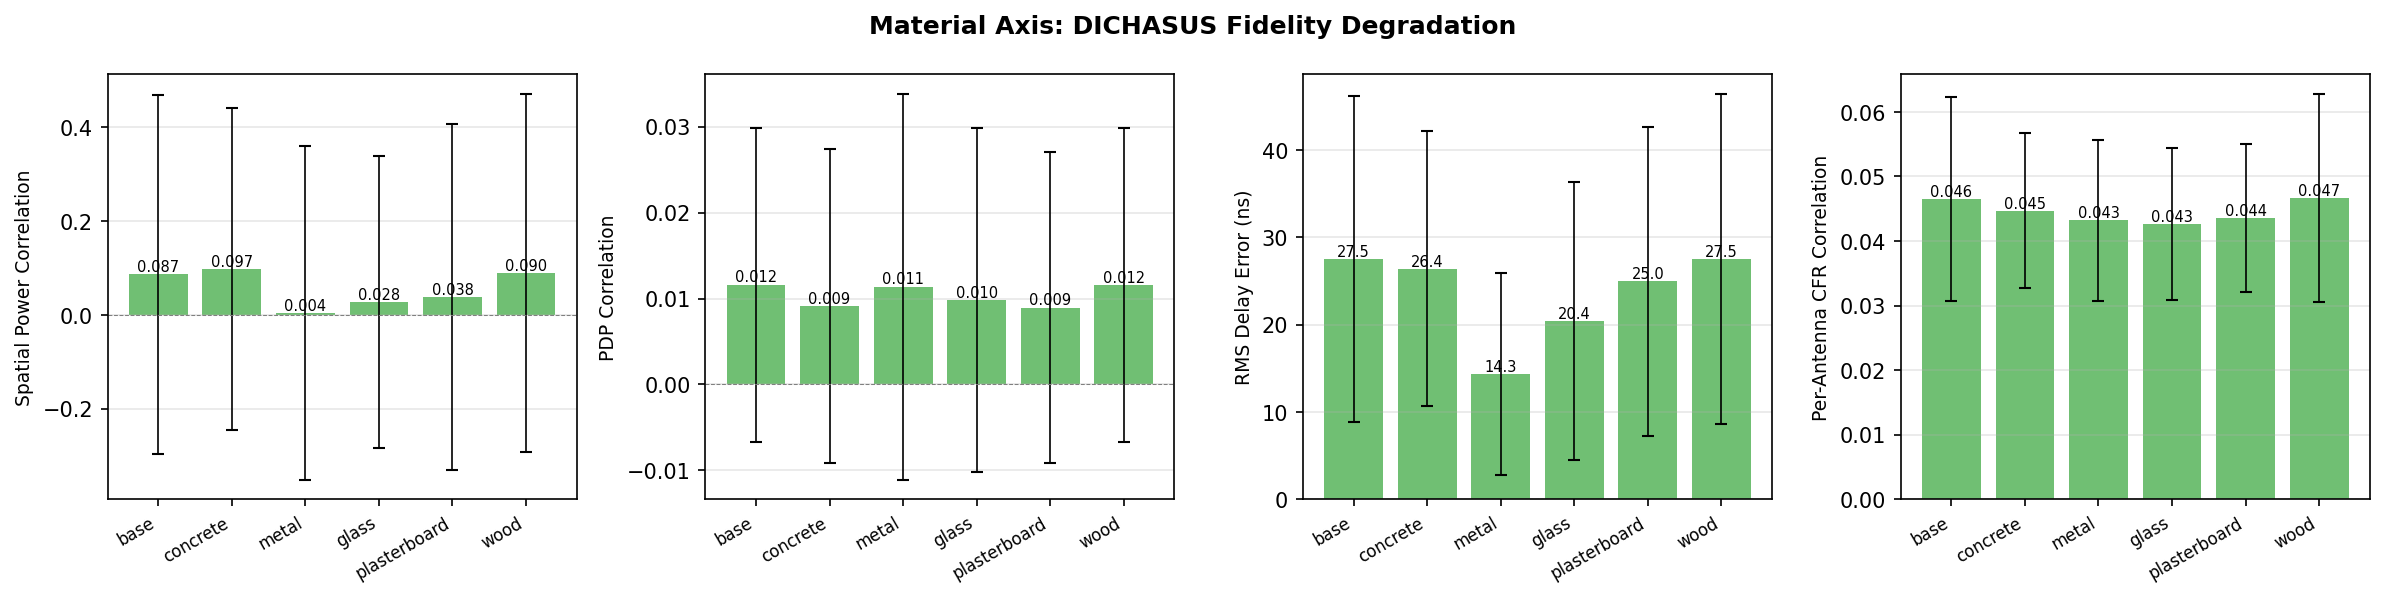
\includegraphics[width=\linewidth,height=0.55\textheight,keepaspectratio]{dichasus_fidelity/material_detail.png}
\end{center}
\end{column}
\begin{column}{0.45\textwidth}
\vspace{0.3cm}
\footnotesize
\begin{tabular}{rcc}
\toprule
\textbf{Material} & \textbf{Pwr Corr} & \textbf{PDP Corr} \\
\midrule
Baseline & $0.087$ & $0.0116$ \\
Concrete & $0.097$ & $0.0091$ \\
Metal & $0.004$ & $0.0114$ \\
Glass & $0.028$ & $0.0098$ \\
Plasterboard & $0.038$ & $0.0089$ \\
Wood & $0.090$ & $0.0116$ \\
\bottomrule
\end{tabular}
\normalsize
\vspace{0.3cm}
\begin{block}{\footnotesize Finding}
\footnotesize
\textbf{Consistent with Canyon}: material choice has limited impact on match quality (all within $\pm 0.05$ of baseline). Metal is the worst ($0.004$) as it over-reflects; wood/concrete closest to baseline. Fine-tuning material parameters is second-order to closing the sim-real gap.
\end{block}
\end{column}
\end{columns}
\end{frame}

%------------------------------------------------

\begin{frame}{\textbf{RT Parameters: Depth and Samples}}
\vspace{-0.2cm}
\begin{columns}[T]
\begin{column}{0.52\textwidth}
\begin{center}
    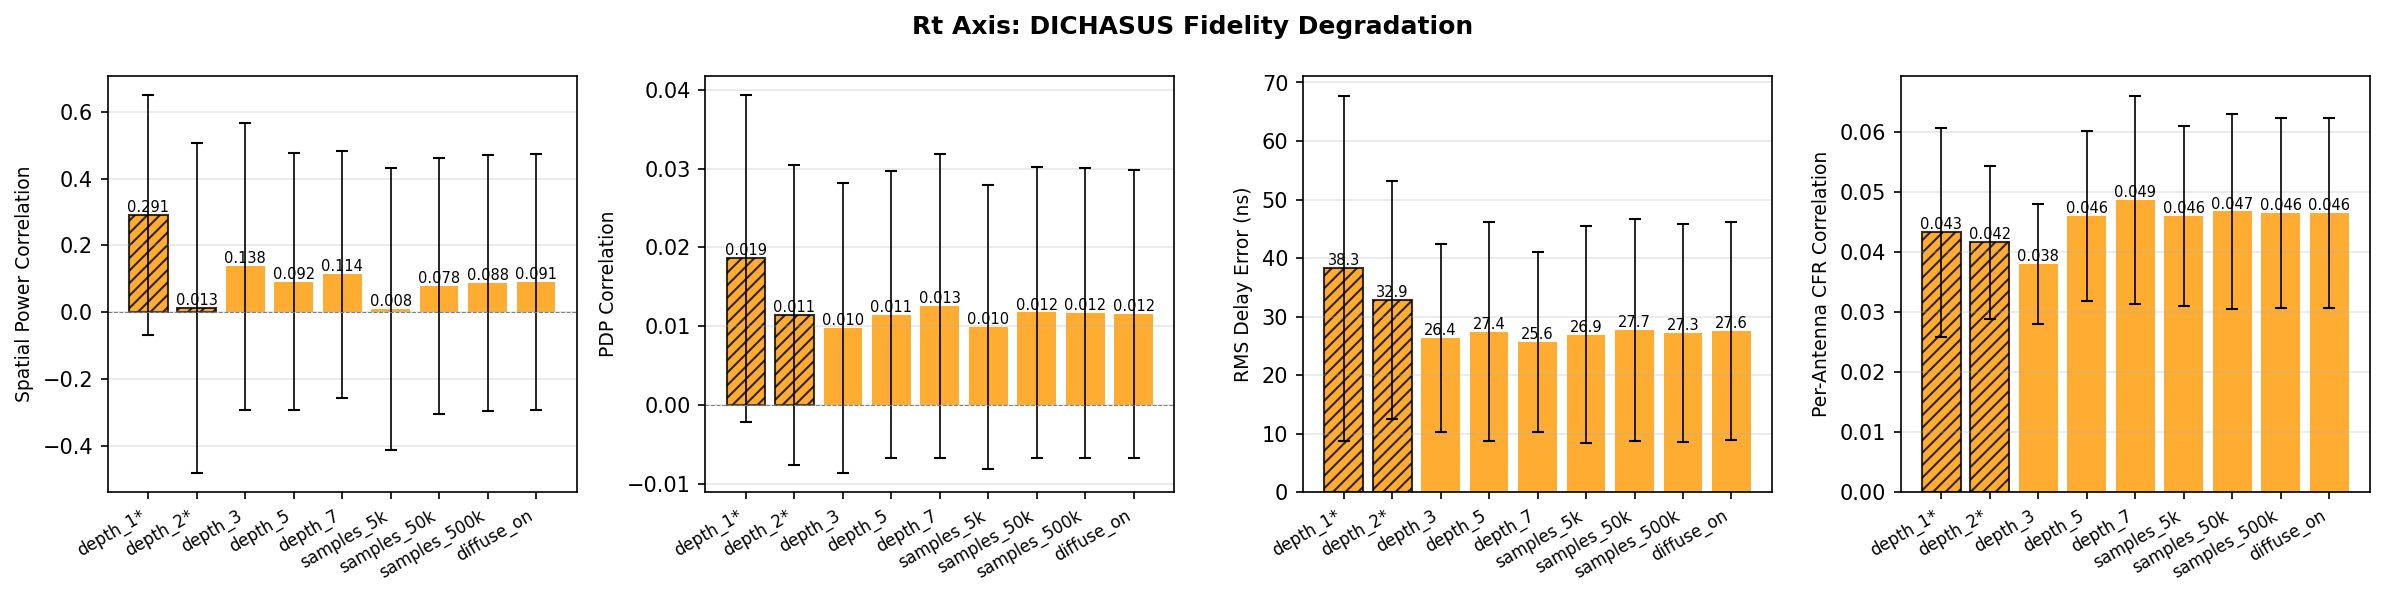
\includegraphics[width=\linewidth,height=0.55\textheight,keepaspectratio]{dichasus_fidelity/rt_detail.png}
\end{center}
\end{column}
\begin{column}{0.45\textwidth}
\vspace{0.1cm}
\scriptsize
\begin{tabular}{rccc}
\toprule
\textbf{RT Config} & \textbf{Pwr} & \textbf{PDP} & \textbf{N} \\
\midrule
depth 1 & $0.291^\dagger$ & $0.0186$ & 15/30 \\
depth 2 & $0.013^\dagger$ & $0.0115$ & 23/30 \\
depth 3 & $0.138$ & $0.0097$ & 30/30 \\
depth 5 & $0.092$ & $0.0115$ & 30/30 \\
depth 7 & $0.114$ & $0.0126$ & 30/30 \\
samples 5k & $0.008$ & $0.0099$ & 30/30 \\
samples 50k & $0.078$ & $0.0118$ & 30/30 \\
samples 500k & $0.088$ & $0.0117$ & 30/30 \\
diffuse on & $0.091$ & $0.0116$ & 30/30 \\
\bottomrule
\end{tabular}
\normalsize
\vspace{0.1cm}
\begin{block}{\footnotesize Finding (with caveat)}
\scriptsize
$^\dagger$\textbf{Depth 1/2 not comparable}: at shallow depth, half the positions yield zero paths and drop out, so averages are over a LoS-dominant subset. Among fair configs (30/30), depth=3 is best (0.14). Samples/diffuse have minor impact at $\geq$50k.
\end{block}
\end{column}
\end{columns}
\end{frame}

%------------------------------------------------

\begin{frame}{\textbf{Hardware: Antenna Configuration}}
\vspace{-0.2cm}
\begin{columns}[T]
\begin{column}{0.52\textwidth}
\begin{center}
    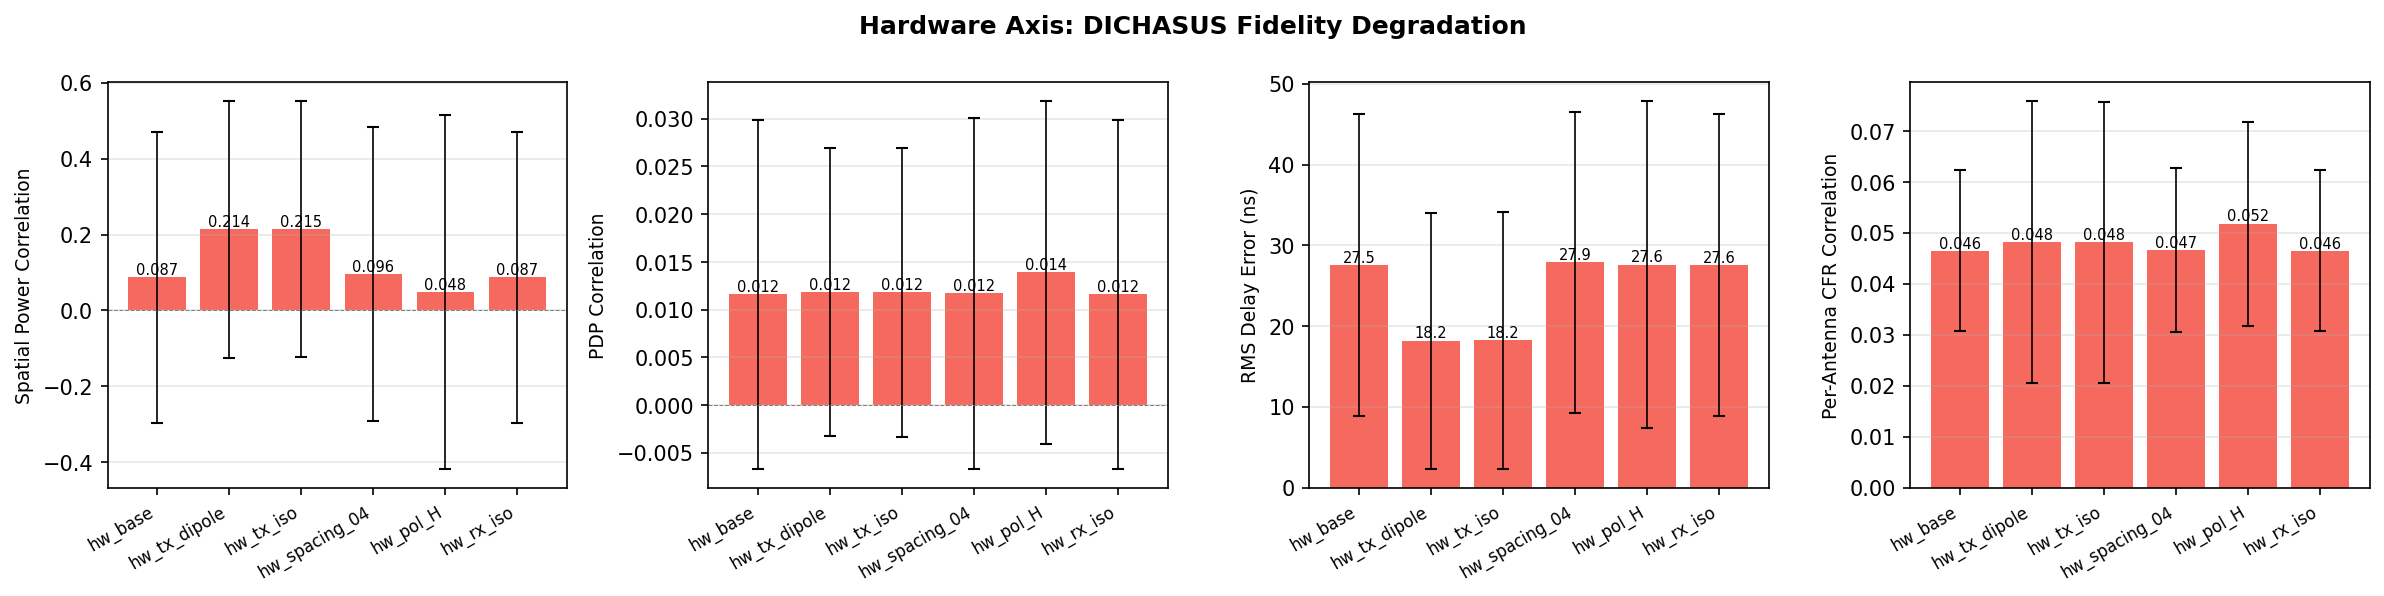
\includegraphics[width=\linewidth,height=0.55\textheight,keepaspectratio]{dichasus_fidelity/hardware_detail.png}
\end{center}
\end{column}
\begin{column}{0.45\textwidth}
\vspace{0.3cm}
\footnotesize
\begin{tabular}{rcc}
\toprule
\textbf{HW Config} & \textbf{Pwr Corr} & \textbf{PDP Corr} \\
\midrule
Baseline & $0.087$ & $0.0116$ \\
Tx Dipole & $0.214$ & $0.0119$ \\
Tx Iso & $0.215$ & $0.0118$ \\
Spacing 04 & $0.096$ & $0.0117$ \\
Pol H & $0.048$ & $0.0139$ \\
Rx Iso & $0.087$ & $0.0116$ \\
\bottomrule
\end{tabular}
\normalsize
\vspace{0.3cm}
\begin{block}{\footnotesize Finding}
\footnotesize
\textbf{Isotropic/dipole TX beat TR38.901} (pwr\_corr 0.21 vs 0.09). Pol.\ H is worst (0.05). Real arrays radiate more uniformly than modeled.
\end{block}
\end{column}
\end{columns}
\end{frame}

%------------------------------------------------
\section{Canyon vs.\ DICHASUS Comparison}
%------------------------------------------------

\begin{frame}{\textbf{Sim-Only vs.\ Real-World: Do Thresholds Hold?}}
\vspace{-0.1cm}
\begin{center}
\small
\begin{tabular}{lccc}
\toprule
\textbf{Axis} & \textbf{Canyon (sim-sim)} & \textbf{DICHASUS (sim-real)} & \textbf{Agree?} \\
\midrule
\textbf{Geometry} & Dominant ($>$10\,dB at 1\,m) & range 0.02--0.12 & \cellcolor{green!15}\checkmark \\
\textbf{Material} & Low impact ($\sim$1.5\,dB) & range 0.00--0.10 & \cellcolor{green!15}\checkmark \\
\textbf{RT Depth} & depth $\geq$3 best & depth=3 best (0.14)$^*$ & \cellcolor{green!15}\checkmark \\
\textbf{RT Samples} & $\geq$5K sufficient & range 0.01--0.09 & \cellcolor{green!15}\checkmark \\
\textbf{HW Pattern} & TR38.901 mandatory & \textbf{dipole/iso best} (0.21) & \cellcolor{red!15}$\times$ \\
\textbf{HW Polarization} & V mandatory & V best (0.09 vs 0.05) & \cellcolor{green!15}\checkmark \\
\bottomrule
\end{tabular}
\end{center}

\vspace{0.1cm}
\begin{block}{Summary}
\footnotesize
Material, geometry, samples, and polarization findings \textbf{transfer} from sim-only to real. But \textbf{antenna pattern} inverts: TR38.901 is predicted optimal in Canyon, yet dipole/iso match DICHASUS better because the measurement arrays radiate more uniformly than the cellular-BS pattern assumed. \\
$^*$depth=1/2 reach only 15/23 positions, so those averages are over an easier LoS-dominant subset and are excluded from the comparison.
\end{block}
\end{frame}

%------------------------------------------------
\section{Material Calibration}
%------------------------------------------------

\begin{frame}{\textbf{Calibration: Closing the Sim-Real Gap}}
\vspace{-0.2cm}
\begin{columns}[T]
\begin{column}{0.48\textwidth}
\begin{block}{Method}
\footnotesize
\begin{itemize}
    \item \textbf{Coordinate descent} over 5 material parameters ($\varepsilon_r$, $\sigma$).
    \item Train on 20 positions from first 2000 (subsample).
    \item Test on positions 2001--3282 (unseen).
    \item Each eval: subprocess RT $\to$ pwr\_corr vs.\ real CSI.
\end{itemize}
\end{block}
\vspace{0.1cm}
\begin{block}{Sim-Real Gap Improvement}
\footnotesize
\begin{tabular}{rcc}
\toprule
& \textbf{Train} & \textbf{Test} \\
\midrule
ITU default & $0.050$ & $0.115$ \\
\rowcolor{green!15} Calibrated & $0.232$ & $\mathbf{0.290}$ \\
\midrule
Improvement & $4.6\times$ & $2.5\times$ \\
\bottomrule
\end{tabular}
\end{block}
\end{column}
\begin{column}{0.48\textwidth}
\vspace{0.1cm}
\footnotesize
\begin{block}{Calibrated Material Parameters}
\scriptsize
\begin{tabular}{rcccc}
\toprule
& \multicolumn{2}{c}{$\varepsilon_r$} & \multicolumn{2}{c}{$\sigma$} \\
\cmidrule(lr){2-3}\cmidrule(lr){4-5}
\textbf{Material} & ITU & Cal. & ITU & Cal. \\
\midrule
Concrete & 5.24 & \textbf{1.5} & 0.121 & 0.05 \\
Glass & 6.31 & \textbf{3.0} & 0.019 & 0.005 \\
Plasterboard & 2.73 & \textbf{4.0} & 0.027 & 0.027 \\
Ceil.\ board & 1.48 & \textbf{25.0} & 0.004 & 0.001 \\
Metal & 1.0 & \textbf{10.0} & $10^7$ & $10^7$ \\
\bottomrule
\end{tabular}
\end{block}
\normalsize
\vspace{0.1cm}
\begin{block}{\footnotesize Key Takeaway}
\footnotesize
Calibration achieves pwr\_corr $= 0.290$ on unseen positions --- \textbf{highest among all 25 configs} and $3.3\times$ better than uncalibrated baseline ($0.087$). Generalizes well to test set.
\end{block}
\end{column}
\end{columns}
\end{frame}

%------------------------------------------------
\section{Diff-RT Calibration}
%------------------------------------------------

\begin{frame}{\textbf{Diff-RT Calibration: Continuous Optimization}}
\vspace{-0.2cm}
\begin{columns}[T]
\begin{column}{0.48\textwidth}
\begin{block}{\footnotesize Motivation: Beyond Grid Search}
\footnotesize
Coordinate descent searches a \textbf{discrete grid}---can we do better with \textbf{continuous optimization}?
\vspace{0.1cm}
\begin{itemize}
    \item Inspired by NVlabs \emph{diff-rt-calibration} (Hoydis et al., 2023).
    \item Joint continuous optimization of all material parameters simultaneously.
    \item Train on 20 positions, test on 30 unseen positions.
    \item Scene: \texttt{inue\_simple} (3 materials).
\end{itemize}
\end{block}
\vspace{0.1cm}
\begin{block}{\footnotesize Refined Parameters}
\scriptsize
\begin{tabular}{rcccc}
\toprule
& \multicolumn{2}{c}{$\varepsilon_r$} & \multicolumn{2}{c}{$\sigma$} \\
\cmidrule(lr){2-3}\cmidrule(lr){4-5}
\textbf{Material} & ITU & Ref. & ITU & Ref. \\
\midrule
Concrete (floor) & 5.24 & \textbf{4.5} & 0.121 & 0.050 \\
Ceil.\ board & 1.48 & 25.0 & 0.004 & 0.001 \\
Plasterboard & 2.73 & \textbf{1.2} & 0.027 & 0.027 \\
\bottomrule
\end{tabular}
\end{block}
\end{column}
\begin{column}{0.48\textwidth}
\begin{block}{\footnotesize Results on Test Set (30 unseen positions)}
\scriptsize
\begin{tabular}{rcc}
\toprule
\textbf{Method} & \textbf{pwr\_corr} & \textbf{pdp\_corr} \\
\midrule
ITU default (dipole) & $0.140$ & $0.015$ \\
Coord descent & $0.105$ & $0.019$ \\
\rowcolor{green!15} \textbf{Refined calibration} & $\mathbf{0.248}$ & $0.015$ \\
\midrule
\textit{Improvement vs ITU} & $1.8\times$ & --- \\
\bottomrule
\end{tabular}
\end{block}
\normalsize
\vspace{0.1cm}
\begin{block}{\footnotesize Key Insight}
\footnotesize
Continuous refinement achieves pwr\_corr $= 0.248$ on \texttt{inue\_simple} (3 objects). The critical change: plasterboard $\varepsilon_r$ from $2.73 \to 1.2$. Wall material dominates because walls have the largest surface area.
\end{block}
\end{column}
\end{columns}
\end{frame}

%------------------------------------------------

\begin{frame}{\textbf{Ablation: What Matters Most After Calibration?}}
\vspace{-0.2cm}
\begin{columns}[T]
\begin{column}{0.48\textwidth}
\begin{block}{\footnotesize Material Ablation}
\footnotesize
Starting from calibrated state (pwr\_corr $= 0.248$), reset each material to ITU default:
\vspace{0.1cm}
\scriptsize
\begin{tabular}{rcc}
\toprule
\textbf{Reset to ITU} & \textbf{pwr\_corr} & \textbf{$\Delta$} \\
\midrule
\rowcolor{green!15} (none --- calibrated) & $0.248$ & --- \\
Reset concrete & $0.254$ & $-0.007$ \\
Reset ceil.\ board & $0.225$ & $+0.022$ \\
\rowcolor{red!15} Reset plasterboard & $0.120$ & $+0.128$ \\
\bottomrule
\end{tabular}
\footnotesize
\vspace{0.2cm}
\begin{block}{\scriptsize Finding}
\scriptsize
\textbf{Plasterboard (walls) dominates}: resetting it destroys $>$50\% of the calibration gain. Concrete barely matters. Ceiling board has moderate impact. $\to$ \textbf{Walls drive the sim-real gap} on this simple scene.
\end{block}
\end{block}
\end{column}
\begin{column}{0.48\textwidth}
\begin{block}{\footnotesize RT \& Antenna Ablation}
\scriptsize
\begin{tabular}{rcc}
\toprule
\textbf{Config (calibrated)} & \textbf{pwr\_corr} & \textbf{N} \\
\midrule
\rowcolor{green!15} Cal + dipole (best) & $\mathbf{0.248}$ & 30 \\
Cal + isotropic & $0.248$ & 30 \\
Cal + TR38.901 & $0.253$ & 30 \\
Cal + diffuse on & $0.248$ & 30 \\
Cal, depth=3 & $0.243$ & 30 \\
Cal, depth=1 & $0.366^\dagger$ & 16 \\
\bottomrule
\end{tabular}
\footnotesize
\vspace{0.1cm}
$^\dagger$Depth=1: only 16/30 reach LoS --- biased high.
\vspace{0.2cm}
\begin{block}{\scriptsize Finding}
\scriptsize
After calibration, \textbf{antenna pattern and diffuse scattering have negligible impact} ($\leq 0.005$ difference). RT depth $\geq$3 is sufficient. The bottleneck is no longer these hyperparameters --- \textbf{material accuracy is the dominant factor}.
\end{block}
\end{block}
\end{column}
\end{columns}
\end{frame}

%------------------------------------------------

\begin{frame}{\textbf{Gradient-Based Calibration (NVlabs Approach)}}
\vspace{-0.2cm}
\begin{columns}[T]
\begin{column}{0.48\textwidth}
\begin{block}{\footnotesize Method: Differentiable Ray Tracing}
\footnotesize
Full NVlabs pipeline (Hoydis et al.\ 2023) adapted for dc41:
\vspace{0.1cm}
\begin{itemize}
    \item Sionna 0.18 + LLVM backend (CPU ray tracing).
    \item Pre-trace paths $\to$ \texttt{compute\_fields} with \texttt{GradientTape}.
    \item \textbf{TrainableMaterials}: learned $\varepsilon_r$, $\sigma$ per object.
    \item \textbf{TrainableAntennaPattern}: mixture of spherical Gaussians.
    \item \textbf{TrainableScatteringPattern}: Lambertian + directive + backscatter.
    \item Loss: SMAPE delay spread + SMAPE power.
    \item 200 positions (120 train, 30 val, 50 test).
\end{itemize}
\end{block}
\end{column}
\begin{column}{0.48\textwidth}
\begin{block}{\footnotesize Results on Test Set (50 positions)}
\scriptsize
\begin{tabular}{rccc}
\toprule
\textbf{Method} & \textbf{pwr\_corr} & \textbf{pdp\_corr} & \textbf{rms err} \\
\midrule
ITU baseline & $0.047$ & $0.557$ & 24.9\,ns \\
Materials only & $0.084$ & $0.567$ & 17.6\,ns \\
Mat + antenna & $0.133$ & $0.560$ & 19.6\,ns \\
\rowcolor{green!15} \textbf{Full (mat+ant+scat)} & $\mathbf{0.167}$ & $\mathbf{0.646}$ & \textbf{17.2}\,ns \\
\midrule
\textit{Coord descent} & $0.248$ & $0.015$ & --- \\
\bottomrule
\end{tabular}
\end{block}
\vspace{0.1cm}
\begin{block}{\footnotesize Key Insight}
\footnotesize
Gradient-based calibration dramatically improves \textbf{PDP correlation} ($0.015 \to 0.646$) --- the multipath structure now matches reality. Scattering learning is critical: adding it jumps pdp\_corr from $0.56$ to $0.65$. RMS delay error drops 31\%.
\end{block}
\end{column}
\end{columns}
\end{frame}

%------------------------------------------------
\section{ML Task: Beam Prediction}
%------------------------------------------------

\begin{frame}{\textbf{Beam Prediction: Sim-to-Real Transfer}}
\vspace{-0.2cm}
\begin{columns}[T]
\begin{column}{0.52\textwidth}
\begin{center}
    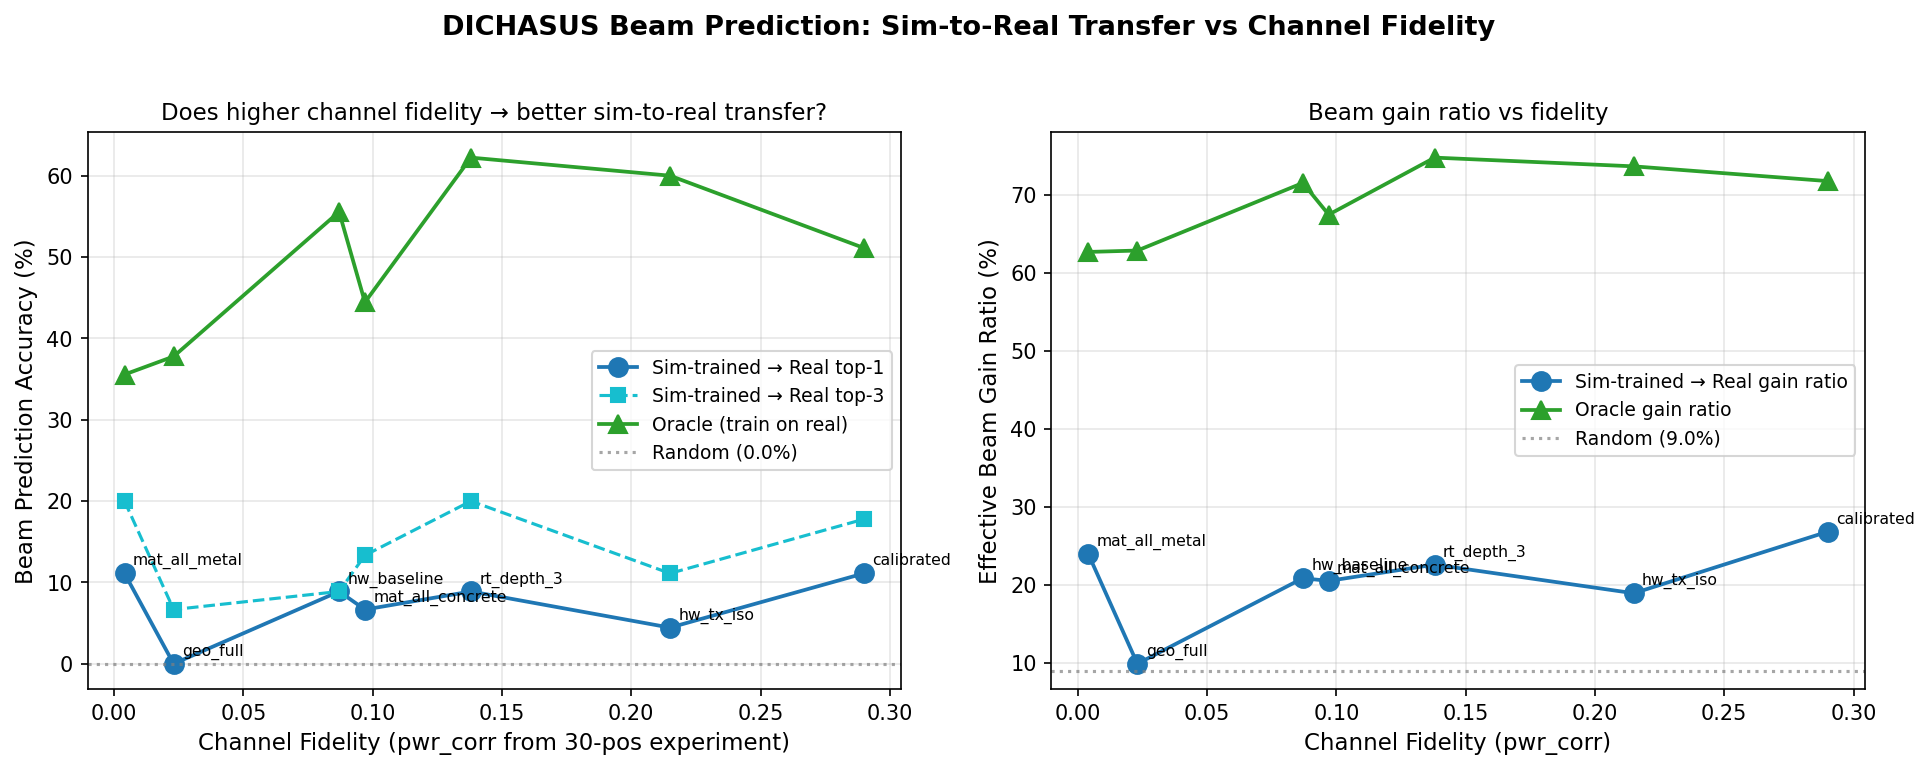
\includegraphics[width=\linewidth,height=0.6\textheight,keepaspectratio]{dichasus_fidelity/beam_pred_vs_fidelity.png}
\end{center}
\end{column}
\begin{column}{0.45\textwidth}
\vspace{0.1cm}
\footnotesize
\textbf{Setup}: MLP maps position $\to$ best DFT beam (64 beams, 32 antennas, array-1). Train on sim labels, test on real labels. 300 positions, 70/15/15 split.
\vspace{0.2cm}

\begin{tabular}{rcccc}
\toprule
\textbf{Config} & \textbf{pwr} & \textbf{Sim} & \textbf{Oracle} \\
& corr & top-1 & top-1 \\
\midrule
\rowcolor{green!15} calibrated & $0.290$ & $11.1\%$ & $51.1\%$ \\
hw\_tx\_iso  & $0.215$ & $4.4\%$  & $60.0\%$ \\
rt\_depth\_3 & $0.138$ & $8.9\%$  & $62.2\%$ \\
mat\_concrete & $0.097$ & $6.7\%$ & $44.4\%$ \\
hw\_baseline & $0.087$ & $8.9\%$ & $55.6\%$ \\
geo\_full    & $0.023$ & $0.0\%$  & $37.8\%$ \\
mat\_metal   & $0.004$ & $11.1\%$ & $35.6\%$ \\
\bottomrule
\end{tabular}
\normalsize
\end{column}
\end{columns}
\end{frame}

%------------------------------------------------

\begin{frame}{\textbf{Beam Prediction: Key Findings}}
\begin{columns}[T]
\begin{column}{0.52\textwidth}
\begin{center}
    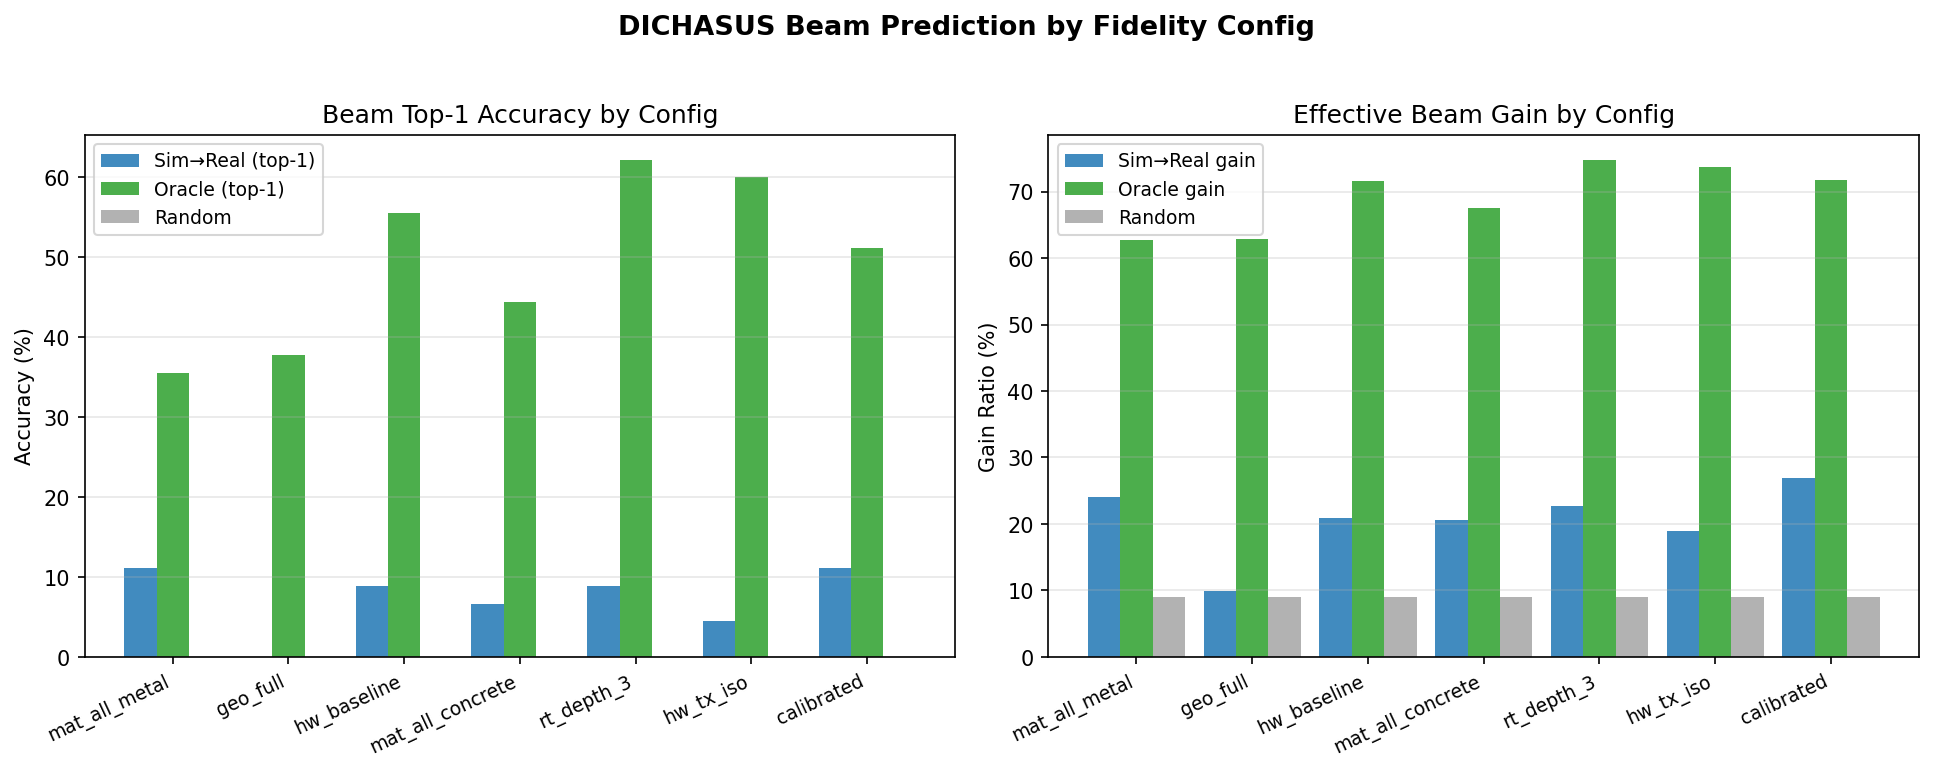
\includegraphics[width=\linewidth,height=0.55\textheight,keepaspectratio]{dichasus_fidelity/beam_pred_per_config.png}
\end{center}
\end{column}
\begin{column}{0.45\textwidth}
\scriptsize
\begin{block}{\scriptsize Finding}
\begin{itemize}
    \item \textbf{Sim-to-real fails} for uncalibrated configs ($\leq 9\%$ top-1 vs.\ random $1.6\%$).
    \item \textbf{Calibration helps}: $11.1\%$ top-1, gain ratio $26.9\%$ (best).
    \item \textbf{Oracle ceiling} $36$--$62\%$: task IS learnable on real data.
    \item \textbf{Weak correlation} pwr\_corr vs ML transfer ($r=0.26$).
    \item Beam label agreement: only $2$--$6\%$ across all configs.
\end{itemize}
\end{block}
\begin{block}{\scriptsize Implication}
With coord-descent calibration, $11\%$ top-1 (vs.\ $51\%$ oracle) shows the gap remains large. Gradient-based calibration with learned scattering improves this further (next slide).
\end{block}
\normalsize
\end{column}
\end{columns}
\end{frame}

%------------------------------------------------

\begin{frame}{\textbf{Beam Prediction: Gradient-Calibrated Channels}}
\vspace{-0.2cm}
\begin{columns}[T]
\begin{column}{0.48\textwidth}
\begin{block}{\footnotesize Setup}
\footnotesize
Same MLP architecture, trained on \textbf{gradient-calibrated} sim channels (Sionna 0.18).
\begin{itemize}
    \item 200 positions, 5-fold cross-validation.
    \item Compare: full calibration vs.\ ITU baseline.
    \item Trained on sim beam labels, tested on real.
\end{itemize}
\end{block}
\vspace{0.1cm}
\begin{block}{\footnotesize K-Fold Sim$\to$Real Results}
\scriptsize
\begin{tabular}{rccc}
\toprule
\textbf{Config} & \textbf{top-1} & \textbf{Gain\%} & \textbf{Oracle} \\
\midrule
\rowcolor{green!15} Grad calibrated & $\mathbf{21.0\%}$ & $\mathbf{45.5\%}$ & $43.5\%$ \\
Grad ITU baseline & $19.5\%$ & $44.9\%$ & $41.0\%$ \\
\midrule
\textit{Coord descent}$^*$ & \textit{11.1\%} & \textit{26.9\%} & \textit{51.1\%} \\
\bottomrule
\end{tabular}
\end{block}
\end{column}
\begin{column}{0.48\textwidth}
\begin{block}{\footnotesize Coarse Beam Prediction (Grad Calibrated)}
\scriptsize
\begin{tabular}{rcc}
\toprule
\textbf{Resolution} & \textbf{Sim$\to$Real} & \textbf{Oracle} \\
\midrule
64 beams (fine) & 21.0\% & 43.5\% \\
16 groups & 27.5\% & 43.5\% \\
\rowcolor{green!15} 8 groups & $\mathbf{31.0\%}$ & 44.5\% \\
\bottomrule
\end{tabular}
\end{block}
\vspace{0.1cm}
\begin{block}{\footnotesize Key Finding}
\footnotesize
Gradient calibration improves sim$\to$real beam prediction by $\sim$8\% relative (21.0\% vs.\ 19.5\%). Direct gain ratio jumps to $\sim$45\% --- calibrated channels capture beam power structure even when fine beam labels differ. Coarse-8 prediction reaches \textbf{31\%}. \\[3pt]
\scriptsize $^*$Coord descent: different split (300 pos, 70/15/15).
\end{block}
\end{column}
\end{columns}
\end{frame}

%------------------------------------------------
\section{Conclusions}
%------------------------------------------------

\begin{frame}{\textbf{Conclusions}}
\footnotesize
\begin{block}{Channel Fidelity (24 uncalibrated configs, 30 positions each)}
\begin{enumerate}
    \item \textbf{Large sim-real gap}: best uncalibrated pwr\_corr $\approx 0.21$ (dipole/iso TX). No config matches real multipath.
    \item \textbf{Antenna pattern matters most}: dipole/iso TX (0.21) beats TR38.901 (0.09). Must match real hardware.
    \item \textbf{Most Canyon rankings transfer}: depth, samples, material, polarization findings hold.
\end{enumerate}
\end{block}

\begin{block}{Calibration: Coordinate Descent $\to$ Gradient-Based}
\begin{enumerate}
    \item Coord descent: pwr\_corr $0.087 \to \mathbf{0.290}$. \textbf{Wall material} ($\varepsilon_r$) dominates.
    \item Gradient-based (NVlabs): pdp\_corr $0.015 \to \mathbf{0.646}$. \textbf{Scattering is critical} for multipath structure.
    \item Complementary gains: coord descent optimizes power profile; gradient optimizes delay structure.
\end{enumerate}
\end{block}

\begin{block}{Beam Prediction Sim$\to$Real Transfer}
\begin{enumerate}
    \item Gradient-calibrated: $\mathbf{21.0\%}$ top-1 (5-fold CV), gain ratio $\mathbf{45.5\%}$, coarse-8 $\mathbf{31\%}$.
    \item Oracle ceiling $\sim$43\%: task is learnable but limited by position-only features.
    \item Calibration consistently improves transfer; gap to oracle suggests room for richer input features.
\end{enumerate}
\end{block}
\normalsize
\end{frame}

%------------------------------------------------

\begin{frame}
\begin{center}
    \Large Questions?
\end{center}
\end{frame}

\end{document}
